\documentclass[10pt]{article}
\usepackage{../../local}
\urlstyle{same}
\usepackage{bbm}
\newcommand{\classcode}{Physics C191}
\newcommand{\classname}{Introduction to Quantum Computing}
\renewcommand{\maketitle}{%
\hrule height4pt
\large{Eric Du \hfill \classcode}
\newline
\large{Lecture Notes} \Large{\hfill \classname \hfill} \large{Whaley, Kolkowitz, Young}
\hrule height4pt \vskip .7em
\small{Header styling inspired by CS 70: \url{https://www.eecs70.org/}}
\normalsize
}
\linespread{1.1}


\begin{document}
	\maketitle
	\section{Introduction}
\subsection{Motivations} 
\begin{itemize}
	\item Why study this class?
		\begin{itemize}
			\item Given a "black box" circuit, with input and output leads, we can determine what's within 
				the "black 
				box".
			\item In this particular case, if our black box contains a voltage divider, and the output voltage is given 
				by the equation:
				\[
				v_{\text{out}}(t) = \frac{R_2}{R_1+ R_2}v_{\text{in}}(t)
				\] 
				In principle though, the signal can be anything that we want: for facial recognition software, the input
				signal could be the configuration of the intensity the camera picks up. There's many more we went over, 
				don't really want to write it all down. 
		\end{itemize}
	\item In essence, there's a lot of systems that can be modeled by a system that takes in a signal \( x(t) \), and 
		outputs a signal \( y(t) = f(x(t))\).
		\begin{itemize}
			\item The signals are usually functions of time, location, in any number of dimensions.
			\item The systems does some sort of transformation on an input signal. In particular, we will study 
				linear systems, shift-invariant systems, etc.
				
				We'll talk about mathematical operations that we use to perform these transformations: Fourier, 
				Laplace, Z-transformations, convolutions, correlation, etc.\item 
	\end{itemize}
\end{itemize}
\subsection{Types of Signals}
\begin{itemize}
	\item \textbf{Continuous-time:} signals defined over continuous variables (e.g. position, time). For 
		instance, a signal \( x(t) \) is continuous for our purposes, since time is a continuous variable. 

		Further, because \( t \) is continuous, then \( x \) must also be continuous.  If the signal is differentiable, 
		then the derivative \( \dv{x(t)}{t} \) also exists. 

		\question{\( t \) being continuous does not imply that \( x(t) \) is continuous (e.g. Thomae function),
		but is it true for this class?} 
	\item \textbf{Discrete-Time:} These are signals defined over discrete variables. For instance, if we had 
		\( x[n] \) as a signal, where \( n \) is an integer. 

		We don't have a concept of differentiability, but we can compute the difference: \( x[n] - x[n- 1] \), and 
		talk about that quantity. 
	\item \textbf{Real-Valued:} A signal \( x(t) \) is real-valued if \( x(t) \in \mathbb R \), where \( \mathbb R \) 
		denotes the set of all real numbers. 
	\item \textbf{Complex-Valued:} A signal \( x(t)  \) is complex-valued if \( x(t) \in \mathbb C \), where 
		\( \mathbb C \) denotes the set of complex numbers. 
	\item Note that while we're using the continuous-time notation here, the same concepts apply with discrete-time 
		signals. 

		\begin{itemize}
			\item Quick recap on complex numbers: denoted by \( a + bj \) or \( a + bi \), where \( i \) and \( j \) 
				denote the imaginary unit. 
			\item They are defined as \( i^2 = -1 \) or \( j^2 = -1 \).
			\item \( a \) is the real part, and \( b \) is the imaginary part. 
			\item We can plot these values in the complex plane, using the real and imaginary representation:
				\begin{center}
					\begin{tikzpicture}
						\draw[-stealth, thick] (-3, 0) -- (3, 0) node[above] {real};
						\draw[-stealth, thick] (0, -3) -- (0, 3) node[above right] {imaginary};
						\draw[red] (0, 0) -- (1.8, 1.4) node[above right, black] 
							{\( z = a + bj \) }; 
						\filldraw[red] (1.8, 1.4) circle (2pt); 
						\draw[dashed] (1.8, 1.4) -- (1.8, 0) node[below] {\( a \) };
						\draw[dashed] (1.8, 1.4) -- (0, 1.4) node[left] {\( b \) };
					\end{tikzpicture}
				\end{center}
				Or using the magnitude-phase representation:
				\begin{center}
					\begin{tikzpicture}
						\draw[-stealth, thick] (-3, 0) -- (3, 0) node[above] {real};
						\draw[-stealth, thick] (0, -3) -- (0, 3) node[above right] {imaginary};
						\draw[red] (0, 0) -- node[midway, above left] {\( m \) } (1.8, 1.4) node[above right, black] 
							{\( z = m\cdot e^{j \theta} \) }; 
						\filldraw[red] (1.8, 1.4) circle (2pt); 
						\draw[red] (1, 0) arc (0:37.87:1) node[midway, right]{\( \theta \) };
						\draw[dashed] (1.8, 1.4) -- (1.8, 0) node[below] {\( m \cdot \cos (\theta) \) };
						\draw[dashed] (1.8, 1.4) -- (0, 1.4) node[left] {\( m \cdot \sin (\theta) \) };
					\end{tikzpicture}
				\end{center}
				We represent the magnitude as \( m = |z| \), and the phase angle \( \theta \) is the angle made 
				with the real axis. 
		\end{itemize}
	\item \textbf{Periodic Signal:} Two quantities we'll introduce here: the period \( T \) is the time it takes 
		for the signal to repeat itself. \( T \) is measured in units of time, generally seconds.
		
		The frequency \( f \) is the "inverse" of period, defined by \( f = \frac{1}{T} \). We will also use 
		the angular frequency \( \omega \), defined by \( \omega = \frac{2\pi}{T} = 2 \pi f \). Angular frequency
		is mainly going to be used when we involve complex numbers. We will see:
		\[
		e^{j \omega t} = e^{j (2 \pi f t)} = \cos(2 \pi ft) + i \sin (2 \pi ft)
		\] 
	\item \textbf{Dimensionality:} We will deal with multi-dimensional signals: an example of a 2D signal are images, 
		which determine the color of a pixel based on a row and column. The spaces that we'll be working with are 
		either \( \mathbb R^{n} \) or \( \mathbb C^{n} \). 
\end{itemize}
\subsection{Signal Transformations}
\begin{itemize}
	\item \textbf{Shifts:} Essentially just shifts the signal along one dimension: \( x(t) \to x(t - T) \). \( T \) 
		is some constant. If  \( T > 0 \), then the shift is to the \textit{right}, and if \( T < 0 \) then 
		the shift is to the \textit{left}.
	\item \textbf{Scaling:} We can multiply a signal \( x(t)  \) by some constant \( a \) : \( x(t) \to a\cdot x(t) \).
		If \( a < 1 \), then we shrink \( x(t) \), and if \(  a > 1 \) then we amplify the signal. 
	\item \textbf{Reversal:} Given \( x(t) \), we can "reverse time" by adding a negative to the argument: \( x(t)
		\to x(-t)\). Visually, all we do is flip the signal around the \( y \)-axis.  
\end{itemize}
\subsection{Signal Properties}
\begin{itemize}
	\item \textbf{Even:} Functions which satisfy \( x(t) = x(-t) \). In other words, if we perform a reversal, the 
		signal stays the same.
	\item \textbf{Odd:} Functions which satisfy \( x(t) = -x(-t) \). If we perform a reversal, the signal becomes the 
		negative of itself.
	\item \textbf{Periodic:} If \( T \) is the period, then \( nT \) is also a period for any \( n \in \mathbb Z \).
		However, we will call \( T \) the fundamental period; the smallest \( T \) for which the function 
		repeats. 

		For the function \( \sin(2 \pi ft) \), the fundamental period is \( 1 / f \).  
\end{itemize}
\subsection{Model Functions}
\begin{itemize}
	\item These are called model functions because they're idealized models to analyze. 
	\item \textbf{Heaviside Step function:} For the continuous-time case it's usually modeled by:
		\[
		u(t) = \begin{cases}
			0 & \text{for \( t < 0 \)}\\
			1 & \text{for \( t \ge 0 \)}
		\end{cases}
		\] 
		In the discrete-time case, it's written as:
		\[
			u[n] = \begin{cases}
				0 & \text{for \( n < 0 \)}\\
				1 & \text{for \(n \ge  0\)}
			\end{cases}
		\] 
\end{itemize}



		
	%\section{More on Model Functions, System Characterization}
\section{Lecture 2}
\subsection{Model Functions Continued}
\begin{itemize}
	\item \textbf{Ramp Function:} The continuous-time is expressed as:
		\[
		r(t) = \begin{cases}
			0 & \text{for \( t < 0 \)}\\
			t & \text{for \( t \ge 0 \)}
		\end{cases}
		\] 
		Similarly in discrete time:
		\[
			\text{ramp}[n] = \begin{cases}
				0 & \text{for \( n < 0 \)}\\
				n & \text{for \( n \ge 0 \)}
			\end{cases}
		\] 
		Note that we can express the ramp function in terms of the step function, in many ways:
		\begin{itemize}
			\item \( r(t) = t \cdot u(t) \)
			\item \( r(t) = \int_{-\infty}^{t}u(t) \diff t \), the discrete case is just a sum over the same bound.
		\end{itemize}
	\item \textbf{Rectangular Function:} In continuous-time:
		\[
		\text{rect}(t) = \sqcap(t) = \begin{cases}
			1 & \text{for \( |t| \le  1 / 2 \)}\\
			0 & \text{else}
		\end{cases}
		\] 
		In discrete time:
		\[
		\text{rect}\left[ \frac{n}{N} \right] = \begin{cases}
			1 & \text{for \( |n| \le  N \)}\\
			0 & \text{for \( |n| > N \)}
		\end{cases}
		\] 
		We can also express \( \text{rect}(t) \) in terms of \( u(t) \) :
		\[
			\sqcap(t) = u\left( t + \frac{T}{2} \right)	- u\left( t - \frac{T}{2} \right) 
		\] 
	\item \textbf{Triangle Function:} In continuous-time:
		\[
		\Lambda(t) = \begin{cases}
			1 - |t| & \text{for \( |t| \le  1 \)}\\
			0 & \text{for \( |t| > 1 \)}
		\end{cases}
		\] 
		And in discrete-time:
		\[
		\Lambda \left[ \frac{n}{N} \right]  = \begin{cases}
			1 - \left|\frac{n}{N}\right| & \text{for \( |n| \le N \)}\\
			0 &\text{else}
		\end{cases}
		\] 
	\item \textbf{Delta Function:} In continuous time, it's called the Dirac delta function. It has the property 
		that \( \delta(t) = 0 \) for all \( t \neq 0  \), but 
		\[
		\int_{-\infty}^{\infty} \delta(t) \diff t  = 1
		\] 
		So in essence, this is an infinitesimally "thin" function, that extends to infinity. There are also 
		other ways to represent the Delta function:
		\begin{itemize}
			\item Derivative of the Heaviside step function: \( \delta(t) = \dv{u(t)}{t} \)
			\item The integral of a complex exponential:
				\[
				\delta(t) = \int_{-\infty}^{\infty} e^{j 2 \pi f t} \diff f = \frac{1}{2\pi}
				\int_{-\infty}^{\infty} e^{j \omega t}\diff  \omega 
				\] 
				\comment{The delta function allows us to approximate the integral \( \int_{-\infty}^{\infty} \cos(\omega t)
				\diff  t\). We can do the following:
				\begin{align*}
					\int_{-\infty}^{\infty} \cos(\omega t) \diff t &= \Re\left[ \int_{-\infty}^{\infty} \cos(\omega t) + 
					i \sin (\omega t)\right] \diff t \\
					&= \Re\left[ \int_{-\infty}^{\infty} e^{i \omega t} \diff  t  \right]  \\
					&= \Re\left[ 2\pi \delta(\omega)  \right]  
				\end{align*}
				Looking at the delta function, we know that when \( \omega = 0 \), then \( \cos(\omega t) = 1 \), so
				the integral diverges, as expected. When \(  \omega \neq 0  \), our integral result implies that 
				the integral evaluates to 0. This is not exactly true since the integral will oscillate 
				between \( \pm 1 \), which is relatively small compared to \( \omega = 0 \), so it can effectively 
				be taken as 0.}
		\end{itemize}
		\question{How does this compare with the definition we use in physics that \( \delta(t) \) is defined as 
			the function which satisfies:
			\[
			\int_{-\infty}^{\infty} f(t) \delta(t) = f(0) 
			\] 
		Do both work?} 

		\answer{See below bullet point, the definition allows you to derive this property.} 
	\item Let's explore some properties of the Delta function: 
		\begin{itemize}
			\item \textbf{Scaling:} 
				\[
					\int_{-\infty}^{\infty} \delta(\alpha t) dt = \int_{-\infty}^{\infty} \delta(t) \dv{\tau}{\alpha}
					= \frac{1}{|\alpha|}
				\] 
				In other words, \( \delta(\alpha t) = \frac{\delta(t)}{|\alpha|} \)
			\item \textbf{Sifting:} If we have \( f(t) \) and multiply it by a Delta function:
				\[
				\int_{-\infty}^{\infty} f(t) \delta(t - T) \diff t = f(T) 
				\] 
			\item \textbf{Delta function of a function:} We can take the delta function of a function as well:
				\[
				\delta(f(t)) = \frac{\delta(t - t_0)}{|f'(t_0)|}, \ f(t_0) = 0
				\] 
				We take the derivative in the denominator. 
		\end{itemize}
	\item In discrete time, the delta function is represented as the Kronecker delta:
		\[
			\delta[n] = \begin{cases}
				1 & n = 0\\
				0 & \text{else}
			\end{cases}
		\] 
		The function attempts to model the Dirac delta but for discrete time intervals:
		\[
			\sum_{n =-\infty}^{\infty}x[n] \delta[n - 10] = x[10]
		\] 
	\item \textbf{Shah function:} It's basically a bunch of Dirac deltas:
		\[
			\text{III}(t) = \sum_{k= 0}^{\infty}\delta(t - k)
		\] 
		In discrete time, it also is a sum of all deltas:
		\[
			\text{III}[n] = \sum_{k = 0}^{\infty}\delta[n - k]
		\] 
\end{itemize}
\subsection{System Characterization} 
\begin{itemize}
	\item Systems perform operations on input signals, like functions \( F: x \to y \). For instance, 
		the following is a moving average filter:
		\[
			y[n] = \frac{1}{3}(x[n - 1] + x[n] + x[n + 1])
		\] 
	\item We will be particularly interested in \textbf{linear systems}, systems which satisfy the following 
		two properties:
		\begin{itemize}
			\item \textbf{Scaling:} If for any input-output pair \( x(t) \to y(t) \), then for any constant \( a \), 
				\( ax(t) \to ay(t) \)
			\item \textbf{Addition:} Given any two input-output pairs 
				\begin{align*}
					x_1(t) &\to y_1(t)\\
					x_2(t) &\to y_2(t)
				\end{align*}
				Then it's also true that \( x_1(t) + x_2(t) \to y_1(t) + y_2(t) \)
		\end{itemize}
		Combining these two properties, given two general signals \( x_1(t) \to y_1(t) \) and \( x_2(t) \to y_2(t) \), 
		then \( ax_1(t) + bx_2(t) \to ay_1(t) + by_2(t)\).

		\comment{Note that a function like \( y(t) = x(t) + b \) is not a linear function, becuase it doesn't 
			satisfy the second property. Even though the function is linear, doesn't mean that the transformation 
		is linear.} 
	\item \textbf{Shift Invariant:} A shift-invariant system is a system where if we shift the input, the output 
		is also shifted. Given \( x(t) \) and its output \( y(t) \), then \( x(t - T) \) should produce 
		 \( y(t -T) \) for any \( T \).
	 \item \textbf{Memoryless:} A function whose output at any given time only depends on the input at that 
		 time. For instance, machine learning algorithms are not memoryless, since their output depends on 
		 previous inputs. 

		 \question{Does "current" here refer to a given input, or does it refer to past inputs? For instance, 
		 is the moving average function considered memoryless?}

		 Most systems that take time to react are not considered memoryless, since 
	 \item \textbf{Causality:} A system is causal if the output depends on the input at the present and past times 
		 only, not on future times. A system defined by:
		 \[
			 y[n] = \frac{1}{3} (x[n] + x[n + 1])
		 \] 
		 is not considered causal, because \( y[n] \) depends on the \( n + 1 \)-th input. 
	 \item \textbf{Stability:} There are many different ways to define stability, here are some of them:
		 \begin{itemize}
		 	\item A system is called BIBO stable if bounded inputs generate boudned 
		 outputs. Mathematically, this means:
		 \[
		 \int_{-\infty}^{\infty} |x(t)|\diff t  < \infty
		 \] 
		 And in discrete time:
		 \[
		 \sum_{-\infty}^\infty |x[n]| < \infty
		 \] 
	 \item We can also look at the energy and power:
		 \[
		 E = \int_{-\infty}^{\infty} |x(t)|^2 \diff t  \ \ P = \lim_{T \to \infty } \int_{-T / 2}^{T / 2} |x(t)|^2 
		 \diff t
		 \] 
		 \end{itemize} 
	 \item \textbf{System Response function:} These are particular outputs for systems when given an impulse 
		 response of a delta function. They are calculated by substituting \( x(t) = \delta(t)  \) in the 
		 continuous case, and \( x[n] = \delta[n] \) in the discrete case. 
		 \question{Watch lecture for this.}

		 To calculate the impulse response for the moving average filter:
		 \[
			 y[n] = \frac{1}{3}(x[n -1] + x[n] + x[n + 1])
		 \] 
		 To find the impulse response, we substitute \( x[n] = \delta[n] \) to get \( h[n] \). Here, notice that 
		 for \( n < -2 \), then \( h[n] = 0 \), since \( x[-2 + 1] = x[-1] = 0 \), and same goes for the other terms. 
		 Then, refer to the following table:
		 \begin{center}
			 \begin{tabular}{c|c}
				 \( n \) & \( h[n] \) \\
				 \hline 
				 -2 & 0 \\
				 -1 & 1/3\\
				 0 & 1/3\\
				 1 & 1/3\\
				 2 & 0
		 	\end{tabular}
		 \end{center}
\end{itemize}

	\section{Characterization Continued}
\subsection{Step Response}
\begin{itemize}
	\item The step response function is the function \( y_{\text{step}}(t) \) when a step function 
		\( u(t) \) is fed into the system. In discrete-time: we feed \( u[n] \) into the system, and get 
		\( y_{\text{step}}[n] \) as an output.
	\item For instance, for the moving average filter defined earlier, we have the following result:
		\begin{center}
			\begin{tabular}{c|c}
				\( n \) &  \( y_{\text{step}}[n] \)\\
				\hline 
				-2 & 0\\
				-1 & 1/3\\
				0 & 2/3\\
				1 & 1\\
				2 & 1
			\end{tabular}
		\end{center}
		Note that this resembles a ramp function, and is called a ramp-step function.
	\item \textbf{Harmonic Response:} The harmonic response is the response by the system when presented with 
		a harmonic function, of the form \( Ae^{i \omega t}\). 

		In discrete time, we feed in \( Ae^{i \omega n} \) where \( n \) is an integer. 
	\item For the moving average filter, let's write out \( y[n] \) :
		\begin{align*}
			y[n] &= \frac{1}{3}\left(Ae^{i \omega (n - 1)} + Ae^{i \omega n} + Ae^{i \omega (n + 1)}\right)\\
			&= \frac{1}{3}\left( e^{-i \omega} + 1 + e^{i \omega} \right)  \\
			&= \frac{1}{3}(2 \cos \omega + 1) Ae^{i \omega n} \\
		\end{align*}
		The interesting thing here is that when given a harmonic function, the system response just scales the signal 
		by a constant amount!
\end{itemize}
\subsection{LCCDE} 
\begin{itemize}
	\item In this class, we will deal with lots of differential equations, so it's going to be very useful to 
		look at their form, and how to solve them.   
	\item There are two solutions to any differential equation: 
		\begin{itemize}
			\item \textbf{Particular Solution:} \( y_p(t) \) is called a particular solution if it satisfies:
				\[
					\sum_{k = 0}^{N}a_k \dv[k]{y_p(t)}{t} = \sum_{k = 0}^{N}b_k \dv[k]{x(t)}{t}
				\] 
			\item \textbf{Homogeneous Solution:} \( y_h(t) \) is called a homogeneous solution if it satisfies:  
				\[
						\sum_{k = 0}^{N}a_k \dv[k]{y_p(t)}{t} =	0
				\] 
		\end{itemize}
	\item In general, the solution will be a linear combination of the two: 
		\[
		y(t) = y_p(T) + ay_h(t)
		\] 
		the value of \( a \) is generally going to be given by some initial condition. 
	\item For the homogeneous solution, an ansats of the form \( Ae^{st} \) where \( s \) is an undetermined constant 
		will solve the differental equation. We can then determine the value of \( s \) by solving the resulting 
		polynomial.

		To determine the value of \( A \), these are determined by the initial conditions, and depending on the 
		number of initial conditions given, that would correspond directly to the number of distinct values of \( A \). 
\end{itemize}


	%\section{Block Diagrams, Linearly Invariant Systems}
\section{Lecture 4}
\subsection{System Block Diagram}
\begin{itemize}
	\item Now we'll look at how to convert an LCCDE into a block diagram. 
	\item Suppose we're given a system of the form
		\[
			\sum_{k = 0}^{N}a_k y[n - k]  = \sum_{k = 0}^{M}b_k x[n - k]
		\] 
		This implies the equation:
		\[
			y[n] = \sum_{k = 0}^{M}\frac{b_k}{a_0}x[n - k] - \sum_{k = 1}^{N}\frac{a_k}{a_0}y[n - k]
		\] 
\end{itemize}
\subsection{Linear Time Invariant (LTI), Linear Shift Invariant (LSI)}
\begin{itemize}
	\item What is an LTI system? Firstly, it's linear, so it satisfies the superposition rule: given 
		two signals \( x_1(t) \) and \( x_2(t) \), then an input of \( ax_1(t) + bx_2(t) \) will generate 
		an output of \( ay_1(t) + by_2(t) \). 
	\item An LSI is also a linear system, and given an input signal \( x(t) \) with an output 
		\( y(t) \), then we can shift
		the system \( x(t - T) \) to generate an output \( y(t - T) \), but \( y(t - T) = y(t) \). In other words, 
		the output will look like \( y(t) \), except shifted by \( T \).  
	\item As an example, the continuous LCCDE is a linear time invariant system. This is because the derivative 
		is linear: 
		\[
			\sum_{k = 0}^{M}\dv[k]{(ax_1(t) + bx_2(t)}{t} = \sum_{k = 0}^{M}b_k \dv[k]{x(t - T)}{(t - T)}
		\] 
		And then we can substitute \( u = t - T \) :
		\[
			\sum_{k = 0}^{M}b_k \dv[k]{x(u)}{u} = \sum_{k = 0}^{M}\dv[k]{y(t - T)}{(t - T)}
		\] 
	\item The same principle also holds for discrete time signals. 
	\item The most important property of an LTI system is that \textbf{the system response is fully characterized 
		by an impulse response function.}

		What this means is that if we feed the system a \( \delta(t) \) or \( \delta[n] \), it gives us an 
		impulse response function \( h(t) \) or \( h[n] \), and this gives us enough information to characterize
		the entire system.
	\item In the continuous time case, suppose we had the following:
		\begin{center}
			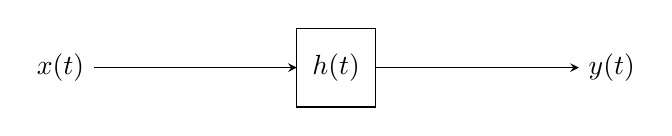
\begin{tikzpicture}
				\node (A) at (-3, 0) {\( x(t) \) };
				\node (B) at (4, 0) {\( y(t) \) };
				\draw[-stealth] (A) -- (0, 0);
				\draw (0, -0.5) rectangle node {\( h(t) \) } (1, 0.5);
				\draw[-stealth] (1, 0) -- (B);
			\end{tikzpicture}
		\end{center}
		Then, \( y(t) \), the signal generated by an arbitrary \( x(t) \) is generated by:
		\[
		y(t) = \int_{-\infty}^{\infty} x(\tau) h(t - \tau) \diff \tau 
		\] 
		In discrete time, the formula is: 
		\[
			y[n] = \sum_{k= -\infty}^{\infty} x[k] h[n - k]
		\] 
		This is called a \textit{convolution}, we will come back to this later. 
\end{itemize}
\subsubsection{Why a convolution?}
\begin{itemize}
	\item Again, consider the diagram:
	\begin{center}
			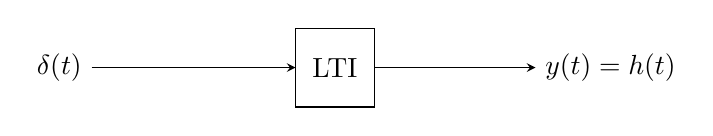
\begin{tikzpicture}
				\node (A) at (-3, 0) {\( \delta(t) \) };
				\node (B) at (4, 0) {\( y(t) = h(t)\) };
				\draw[-stealth] (A) -- (0, 0);
				\draw (0, -0.5) rectangle node {LTI } (1, 0.5);
				\draw[-stealth] (1, 0) -- (B);
			\end{tikzpicture}
		\end{center}
		If we send a signal \( \delta(t - \tau) \) into the system, then due to linear time invariance, the 
		system should output \( y(t - \tau) = h(t - \tau) \). 
	\item If we now send the signal \( x(\tau) \delta(t - \tau) \), then because \( x(\tau) \) is a constant, 
		then we invoke linearity to get that the output is  \( x(\tau) h(t - \tau) \). 
	\item Now, consider what happens when we send in the signal that is just a combination of all possible \( \tau \). 
		Each \( x(\tau) \) is a constant, so the output signal is of the form
		\[
		\int_{-\infty}^{\infty} x(\tau) \delta(t - \tau) \mapsto \int_{-\infty}^{\infty} x(\tau) h(t - \tau) 
		\diff \tau
		\] 
		But now notice that this signal can also be written as:
		\[
		\int_{-\infty}^{\infty} x(\tau) \delta(t - \tau) \diff \tau = x(t)
		\] 
		And so if we're sending in a signal \( x(t) \), then the output should be \( y(t) \)! Thus, we've proven that
		the impulse response is all we need in order to characterize \( y(t) \).
	\item For future reference, a convolution, denoted by \( x(t) * h(t) \), is defined as: 
		\[
		x(t) * h(t) = \int_{-\infty}^{\infty} x(\tau) h(t - \tau) \diff  \tau = \int_{-\infty}^{\infty} x(t - \tau)
		h(\tau) \diff \tau
		\] 
		this last equality shows that convolution is a commutative operation. 
\end{itemize}
\subsubsection{Impulse Response of 1st order LCCDE}
\begin{itemize}
	\item Recall the step response to LCCDE:
		\[
			\dv{y(t)}{t} + ay(t) = bx(t) = bu(t) \implies y_{\text{step}}(t) = 
			\left( \frac{b}{a}( 1 - e^{-at}) \right) u(t)
		\] 
	\item Given an impulse, which in this case can be written as: 
		\[
		\delta(t) = \lim_{\epsilon \to 0}\frac{u(t) - u(t - \epsilon)}{\epsilon}
		\] 
		This implies that the response \( h(t) \) is given by: 
		\[
		h(t) = \lim_{\epsilon \to 0 }\frac{y_{\text{step}}(t) - y_{\text{step}}(t - \epsilon)}{\epsilon} 
		= \lim_{\epsilon \to 0}
		\frac{\frac{b}{a}\left( e^{-a(t - \epsilon)}u(t - \epsilon) - e^{-at}u(t) \right) }{\epsilon}
		= be^{-at}u(t)
		\] 
		(verify this at home, the simplification makes use of the fact that \( e^{a\epsilon} \approx 
		1 + a\epsilon + a^2 \frac{\epsilon^2}{2} + \cdots\), but the higher order terms die).
\end{itemize}
\subsection{Harmonic Response of an LTI system}
\begin{itemize}
	\item The response of an LTI system to a complex signal \( x(t) = Ae^{j \omega t} \) is always going to be another 
		complex exponential signal \( y(t) = H(\omega) Ae^{j \omega t} \)
	\item Given the input signal \( x(t) = Ae^{j \omega t} \), we can write:
		\begin{align*}
			y(t) &= \int_{-\infty}^{\infty} x(\tau) h(t - \tau) \diff \tau\\
				 &= \int_{-\infty}^{\infty} Ae^{j \omega t}
			h(t - \tau) \diff \tau \\
				 &= \int_{-\infty}^{\infty} Ae^{j \omega (t - \tau')}h(\tau') \diff \tau'\\
				 &= Ae^{j \omega t}\underbrace{\int_{-\infty}^{\infty} e^{-j \omega \tau'}h(\tau') \diff \tau'}_{
				 H(\omega)}\\
				 &= H(\omega) Ae^{j \omega t} 
		\end{align*} 
	\item By definition:
		\[
		H(\omega) \equiv \int_{-\infty}^{\infty} e^{-j \omega \tau'}h(\tau') \diff \tau' \ \ 
		H(f) \equiv \int_{-\infty}^{\infty} e^{-j 2 \pi ft}h(t) \diff t 
		\] 
		You'll recognize \( H(\omega) \): it's the Fourier transform equation.
		
		\question{When given an harmonic input, and we're asked to measure it, are we measuring the real part 
		of the signal?}
\end{itemize}
\subsubsection{Example: Frequency response of an RC Circuit}
\begin{itemize}
	\item Given the following circuit:
		% insert circuitkkz
	\item The impulse response is given by the differential equation:
		\[
			\dv{y(t)}{t} + \frac{1}{RC}y(t) = \frac{1}{RC}x(t)
		\] 
		This is a first order LCCDE, so therefore the impulse response \( h(t) \) is given by 
		\( h(t) = be^{-at}u(t) \). 
	\item For the frequency response, we have a function of the form \( x(t) = e^{j \omega t} \), 
		which we know has an output signal of the form \( y(t) = H(\omega) e^{j \omega t} \). So all that remains
		now is to find \( H(\omega) \) :
		\begin{align*}
			y(t) &= e^{j \omega t }\int_{-\infty}^{\infty} e^{-j \omega t}h(\tau) \diff  \tau \\
			&= e^{j \omega t}\int_{-\infty}^{\infty} be^{-a\tau}u(\tau) e^{-j \omega \tau}\diff \tau  \\
			&= be^{j \omega t}\int_{0}^{\infty} e^{-a \tau}e^{-j \omega \tau}\diff \tau  \\
			&= \left( \left.-\frac{1}{a + j \omega}e^{-a \tau}e^{-j \omega t}\right|_0^{\infty}\right)
				be^{j \omega t} \\
				&= \frac{b}{a + j \omega}e^{j \omega t} 
		\end{align*}
		Now, if we impose that \( a = b = \frac{1}{RC} \), then we get the equation: 
		\[
		\frac{\frac{1}{j c \omega}}{\frac{1}{j c \omega} + R}e^{ j \omega t}
		\] 
		Now, \( \frac{1}{jc\omega} \) is the impedance of a capacitor, and this overall equation takes the form of a 
		voltage divider for a circuit with known impedance: 
		\[
		y(t) = \frac{z(\omega)}{z(\omega) + R}e^{j \omega t}
		\] 
\end{itemize}
\subsection{Sinusoidal Input} 
\begin{itemize}
	\item With the harmonic response tools, we can now evaluate the system response when given a sinusoidal 
		input, since we know that 
		\[
		\cos(\omega t) = \frac{e^{ j \omega t} + e^{- j \omega t}}{2}
		\] 
		\question{Does the same work with sine, where there's a complex number is in the denominator?} 
\end{itemize}
\subsection{LTI systems in Parallel and Series}
\begin{itemize}
	\item For a basic system with a single input and output, 
		we've already discussed that \( y(t) = x(t) * h(t) \). Now, what if we connect these systems in 
		parallel?
		\begin{center}
			\begin{tikzpicture}
				\node (A) at (-3, 0) {\( x(t) \) };
				\node (B) at (4, 0) {\( y(t) \) };
				\node (C) at (1.5, 0) {+};
				\draw[-stealth] (A) -- (-0.5, 0) -- (-0.5, 1) -- (0, 1);
				\draw (0, 0.5) rectangle node {\( h_1(t) \) } (1, 1.5);
				\draw[-stealth] (-0.5, 0) -- (-0.5, -1) -- (0, -1);
				\draw (0, -0.5) rectangle node {\( h_2(t) \) } (1, -1.5);
				\draw[-stealth] (1, 1) -- (1.5, 1) -- (C);
				\draw (C) circle (0.2cm);
				\draw[-stealth] (C) -- (B);
				\draw[-stealth] (1, -1) -- (1.5, -1) -- (C);
			\end{tikzpicture}
		\end{center}
		then, the result \( y(t) \) is given by \( y(t) = x(t) * h_1(t) + x(t) * h_2(t) = x(t) * 
		(h_1(t) + h_2(t))\).
	\item If we connect them in series: 
		\begin{center}
			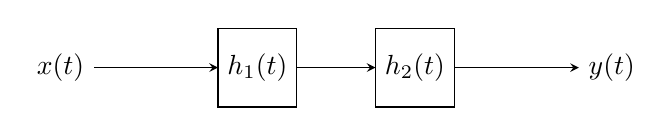
\begin{tikzpicture}
				\node (A) at (-3, 0) {\( x(t) \) };
				\node (B) at (4, 0) {\( y(t) \) };
				\draw[-stealth] (A) -- (-1, 0);
				\draw (-1, -0.5) rectangle node {\( h_1(t) \) } (0, 0.5);
				\draw[-stealth] (0, 0) -- (1, 0);
				\draw (1, -0.5) rectangle node { \( h_2(t) \) } (2, 0.5);
				\draw[-stealth] (2, 0) -- (B);
			\end{tikzpicture}
		\end{center}
		then	
\end{itemize}

	\section{Polynomial Multiplication II}
\begin{itemize}
	\item As a recap, we have two polynomials \( p \) and \( q \), both of degree \(  n -1 \), and we want to multiply 
		them. 
	\item We saw the \textit{coefficient representation}, where we specify its coefficients. So for \( p \), we have \( (p_0, p_1, 
		\dots, p_{n-1})\). Last lecture, we saw \( O(n^2) \) algorithm to multiply the polynomials using the 
		coefficient representation.
	\item We also saw the \textit{value representation}, where instead of giving the polynomial itself we give a set of 
		\( m \) points that the polynomial passes through. As long as \( m \ge  n \), then this set of points 
		fully specifies the polynomial. With this representation, we saw that polynomials can be multiplied in \( O(n) \) time. 
	\item So our main question was: is there a way for us to use the value representation to speed up the coefficient 
		representation multiplication?
	\item Roots of unity: the set of points we will evaluate our polynomials on. 
\end{itemize}
\subsection{Fast Fourier Transform}
\begin{itemize}
	\item Input: \( m \), a power of 2, a \( p(x) = p_0 + p_1x + \cdots + p_{m-1}x^{m-1} \). Our goal is to evaluate 
		 \( p( \omega_0), p(\omega_1), \dots, p(\omega_{m - 1}) \). 
	 \item We will use a divide and conquer approach:
		 \begin{center}
		 	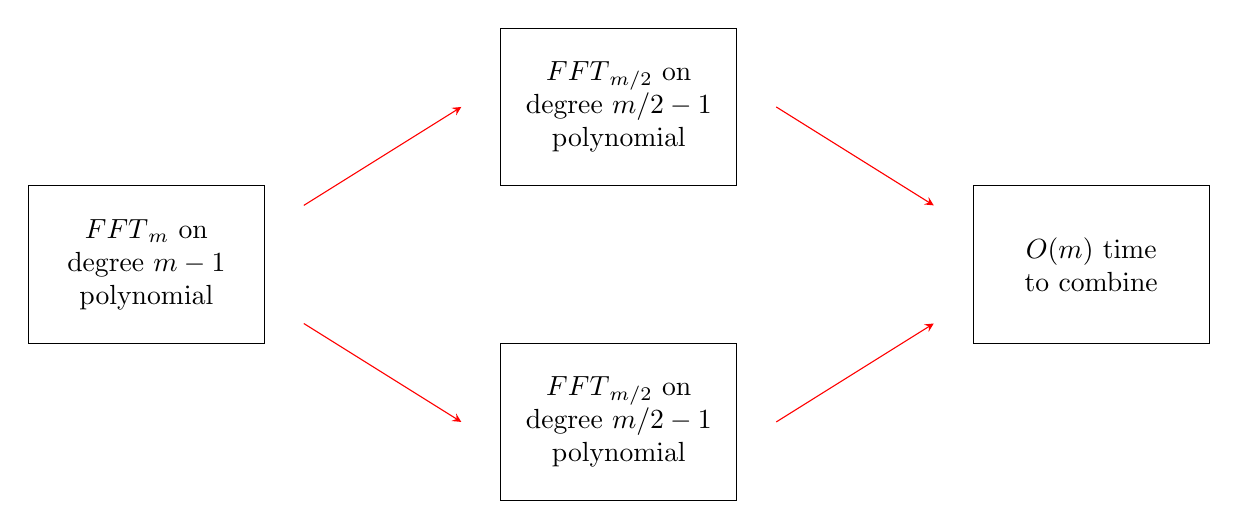
\begin{tikzpicture}[every text node part/.style={align=center}]
		 		\draw(0, -1) -- (3, -1) -- (3, 1) -- (0, 1) -- cycle;
				\draw(6, 1) -- (9, 1) -- (9, 3) -- (6, 3) -- cycle;
				\draw(6, -1) -- (9, -1) -- (9, -3) -- (6, -3) -- cycle;
				\draw(12, -1) -- (15, -1) -- (15, 1) -- (12, 1) -- cycle;
				\draw node at (1.5, 0) {\( \text{FFT}_m \) on \\degree \( m - 1 \) \\ polynomial}; 
				\draw node at (7.5, 2) { \( \text{FFT}_{m / 2} \) on \\ degree \( m / 2 - 1 \) \\ polynomial};
				\draw node at (7.5, -2) { \( \text{FFT}_{m / 2} \) on \\ degree \( m / 2 - 1 \) \\ polynomial};
				\draw node at (13.5, 0) {\( O(m) \) time \\ to combine};
				\draw[-stealth, red] (3.5, 0.75) -- (5.5, 2);
				\draw[-stealth, red] (3.5, -0.75) -- (5.5, -2);
				\draw[-stealth, red] (9.5, 2) -- (11.5, 0.75);
				\draw[-stealth, red] (9.5, -2) -- (11.5, -0.75); 
		 	\end{tikzpicture}
		 \end{center}
		 This will give us a recurrence relation \( T(m) \le  2 \cdot T(m / 2) + O(m) \), and from the master theorem this 
		 gives an \( O(m \log m) \) runtime.
\end{itemize}
\subsection{Divide and Conquer}
\begin{itemize}
	\item To figure out how to divide, let's first write out \( p(x) \) :
		\[
		p(x) = p_0 + p_1x + p_2x^2 + p_3x^3 + \cdots
		\] 
		Let's split \( p \) into two parts, based on the parity of the exponent. We'll call these the even and odd 
		halves:
		\begin{align*}
			p_E(x) &= p_0 + p_2x^2 + p_4x^{4} + \cdots + p_{m - 2}x^{m - 2}\\
			p_O(x) &= p_1x + p_3x^3 + \cdots + p_{m - 1} x^{m - 1} 
		\end{align*}
		But notice that we can rewrite the even part a little bit:
		\[
		p_E(x) = p_0 + p_2(x^2) + p_4(x^2)^2 + p_6(x^2)^3 + \cdots = \text{Even}(x^2)
		\] 
		But this looks like a polynomial with coefficietns \( p_0, p_2, p_4, \dots \) evaluated on \( x^2 \)! We will call 
		this polynomial \( \text{Even}(z) \). For the odd part, we factor out an \( x \) :
		\[
		p_1x + p_3x^3 + \cdots = x(p_1 + p_3x^2 + p_5x^{4} + \cdots) = x \cdot \text{Odd}(x^2)
		\] 
		The key to note here is that we have a recursion in the fact that we can express the evaluation of the polynomials 
		at the \( n \)-th step as a computation involving another polynomial but evaluated on \( x^2 \). So, we have 
		\[
		p(x) = \text{Even}(x^2) + x \cdot \text{Odd}(x^2)
		\] 
		The degree of the even part is \( (m - 2) / 2 = m / 2 - 1 \), and the same goes for odd part.   
	\item Now if we want to compute \( p \) on \( \omega_i \), then we have \( p(\omega_i) = \text{Even}(\omega_i^2) + 
		\omega_i \cdot \text{Odd}(\omega_i^2)\). 
	\item Because we are squaring the arguments, then this means that we are evaluating the Even and Odd parts on the 
		\( m / 2 \)-th roots of unity, because of our magical fact!
	\item So to compute \( p(\omega_i) \), we recursively evaluate the even and odd parts at the  \( m / 2 \)-th roots of unity:
		\( \alpha_0, \alpha_1, \dots, \alpha_{m / 2 - 1} \). 
	\item To combine, all we need to do is multiply the odd part by  \( \omega_i \), then add the two parts together. So, the 
		combination step only takes \( O(m) \) work. So this fully gives our recursion \( T(m) \le  2 \cdot T(m / 2) + O(m) \), 
		hence the \( O(m \log m) \) runtime. 
\end{itemize}
\subsection{Fast Interpolation}
\begin{itemize}
	\item An update on our algorithm scheme:
		\begin{center}
			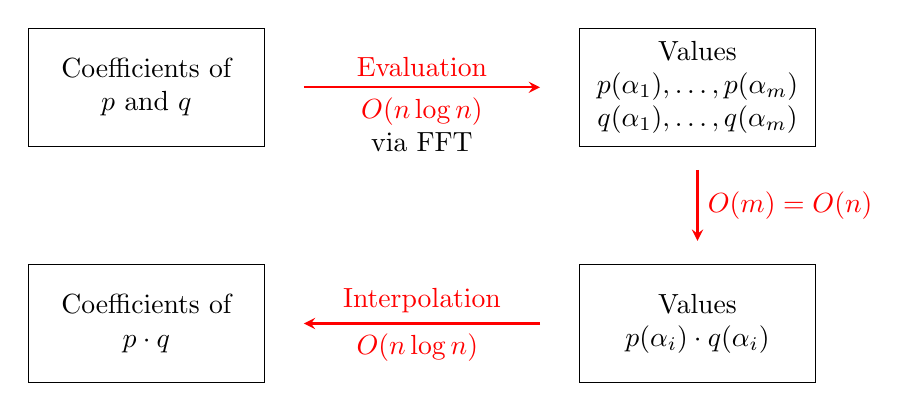
\begin{tikzpicture}[every text node part/.style={align=center}]
				\foreach \x in {0, 7}
				\foreach \y in {0, 3}
				{
					\draw (\x, \y) -- (\x+3, \y) -- (\x+3, \y+1.5) -- (\x, \y+1.5) -- cycle;
				}
				\draw node at (1.5, 0.75) {Coefficients of \\ \( p \cdot q \)};
				\draw node at (1.5, 3.75) {Coefficients of \\ \( p \) and \( q \) };
				\draw node at (8.5, 0.75) {Values \\ \( p(\alpha_i) \cdot q(\alpha_i) \) };
				\draw node at (8.5, 3.75) {Values \\ \( p(\alpha_1), \dots, p(\alpha_m) \) \\ \( q(\alpha_1), \dots, q(\alpha_m) \) };
				\draw[-stealth, red, thick] (3.5, 3.75) --node[midway, above] {Evaluation} node[midway, below] 
					{\( O(n \log n) \) \\ \textcolor{black}{via FFT}} (6.5, 3.75); 
				\draw[-stealth, red, thick] (8.5, 2.7) -- node[midway, right] {\( O(m) = O(n) \) } (8.5, 1.8);
				\draw[-stealth, red, thick] (6.5, 0.75) -- node[midway, above] {Interpolation} node[midway, below] 
					{\( O(n \log n) \) } (3.5, 0.75);
			\end{tikzpicture}
		\end{center}
	\item Now we want to figure out the interpolation step: given \( r(\omega_0), r(\omega_1), \dots, r(\omega_{m - 1}) \), we want 
		to get back the coefficient representation of \( r(x) \). This is called the inverse FFT. 
	\item It turns out that when we do the Fourier transform, we basically get the inverse Fourier transform for free. Recall 
		the Fourier transform:
		\[
			p(\omega_\ell) = \sum_{j = 0}^{m - 1}p_j (\omega_\ell)^{j}
		\]
		This equation comes from replacing all \( x \) 's with \( \omega_\ell \). Then, the inverse Fourier transform is written 
		as follows:
		\[
			p_{\ell} = \frac{1}{m} \cdot \sum_{j = 0}^{m - 1}p(\omega_j) \cdot (\omega_{m - \ell})^{j} = \frac{1}{m} \cdot 
			q(\omega_{m - \ell})
		\] 
		Here, \( q(x) = p(\omega_0) + p(\omega_1)x + \cdots p(\omega_{m - 1})x^{m - 1} \). So in essence, this is basically another 
		polynomial evaluation, which we already know happens in \( O(m \log m) = O(n \log n) \) time!
	\item So, now let's look at the completed diagram:
		\begin{center}
			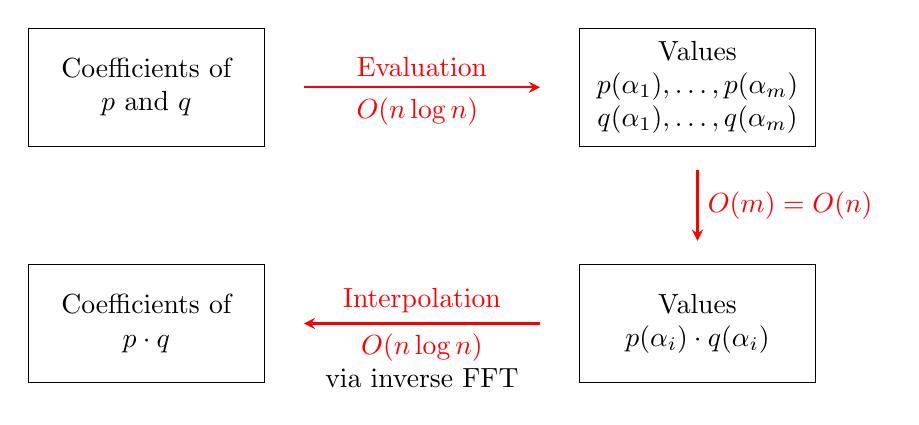
\begin{tikzpicture}[every text node part/.style={align=center}]
				\foreach \x in {0, 7}
				\foreach \y in {0, 3}
				{
					\draw (\x, \y) -- (\x+3, \y) -- (\x+3, \y+1.5) -- (\x, \y+1.5) -- cycle;
				}
				\draw node at (1.5, 0.75) {Coefficients of \\ \( p \cdot q \)};
				\draw node at (1.5, 3.75) {Coefficients of \\ \( p \) and \( q \) };
				\draw node at (8.5, 0.75) {Values \\ \( p(\alpha_i) \cdot q(\alpha_i) \) };
				\draw node at (8.5, 3.75) {Values \\ \( p(\alpha_1), \dots, p(\alpha_m) \) \\ \( q(\alpha_1), \dots, q(\alpha_m) \) };
				\draw[-stealth, red, thick] (3.5, 3.75) --node[midway, above] {Evaluation} node[midway, below] 
					{\( O(n \log n) \) } (6.5, 3.75); 
				\draw[-stealth, red, thick] (8.5, 2.7) -- node[midway, right] {\( O(m) = O(n) \) } (8.5, 1.8);
				\draw[-stealth, red, thick] (6.5, 0.75) -- node[midway, above] {Interpolation} node[midway, below] 
					{\( O(n \log n) \) \\ \textcolor{black}{via inverse FFT}} (3.5, 0.75);
			\end{tikzpicture}
		\end{center}
		So this shows that polynomial multiplication can be done in \( O(n \log n) \) time!  
\end{itemize}
\subsection{The Matrix Viewpoint}
\begin{itemize}
	\item There's another way to represent \( p(x) \), as a column vector:
		\[
		\begin{bmatrix} p(\omega_0)\\p(\omega_1)\\p(\omega_2)\\ \vdots \\ p(\omega_{m - 1}) \end{bmatrix} = 
		\begin{bmatrix} p_0 + p_1\omega_0 + p_2 \omega_0^2 + \cdots + p_{m-1}\omega_0^{m- 1}\\
		p_0 + p_1 \omega_1 + p_2\omega_1^2 + \cdots + p_{m-1}\omega_1^{m-1}\\
	\vdots \\
p_0 + p_1\omega_{m-1} + p_2\omega_{m-1}^2 + \cdots+ p_{m-1}\omega_{m-1}^{m-1}\end{bmatrix} 
= \underbrace{\begin{bmatrix} 1 & \omega_0 & \omega_0^2 & \dots & \omega_0^{m-1}\\
1 & \omega_1 & \omega_1^2 & \dots & \omega_1^{m-1}\\
1 & \omega_2 & \omega_2^2 & \dots & \omega_2^{m-1}\\
\vdots & \vdots & \vdots & \ddots & \vdots\\
1 & \omega_{m-1} & \omega_{m-1}^2 & \dots & \omega_{m-1}^{m-1}\end{bmatrix}}_{M} \cdot \underbrace{\begin{bmatrix} p_0\\p_1\\p_2\\ \vdots \\p_{m-1} \end{bmatrix}}_{[p]} 
		\] 
	\item If we didn't know FFT, then this computation is just a matrix multiplied by a vector, whihc would take \( O(m^2) \)  
		time. However, FFT basically gives us a way to compute this matrix in \( O(m \log m) \) time!

		Note also that this also solves this \textbf{without ever writing down \( M \) !} 
	\item The Inverse FFT looks much cleaner in this representation:
		\[
		M^{-1} \cdot \begin{bmatrix} p(\omega_0)\\p(\omega_1)\\p(\omega_2)\\ \vdots \\ p(\omega_{m-1}) \end{bmatrix} = 
		\begin{bmatrix} p_0\\p_1\\p_2\\ \vdots \\ p_{m-1} \end{bmatrix} 
		\] 
	\item For \( M \) specifically, we have \( M_{ij} = \omega_i^{j} = (\omega_1^{i})^{j} = \omega_1^{ij} \). Then, the inverse 
		is defined as: \( (M^{-1})_{ij} = \frac{1}{n} \cdot \omega_{m-i}^{j} \). 
\end{itemize}
\subsection{Applications}
\begin{itemize}
	\item \textbf{Cross Correlation:}
		Given the product of \( p(x) = p_0 + p_1x + p_2x^2 + p_3x^3 \) and \( q(x) = q_0 + q_1x + q_2x^2 + q_3x^3 \), the 
		coefficient on \( x^{i} \) in \( p(x) \cdot q(x) \) is
		\[
		p_0q_{i} + p_1q_{i-1} + \cdots + p_{i-1}q_{1} + p_{i}q_0
		\] 
		Now consider two arrays \( [p_0, p_1, p_2, p_3] \) and \( [q_3, q_2, q_1, q_0] \). Now let's stack them on top of each 
		other and take the dot product of the overlap. Depending on where they overlap, it actually corresponds to the coefficient 
		on some \( x^{i} \) in \( p(x) \cdot q(x) \).  
		\begin{center}
			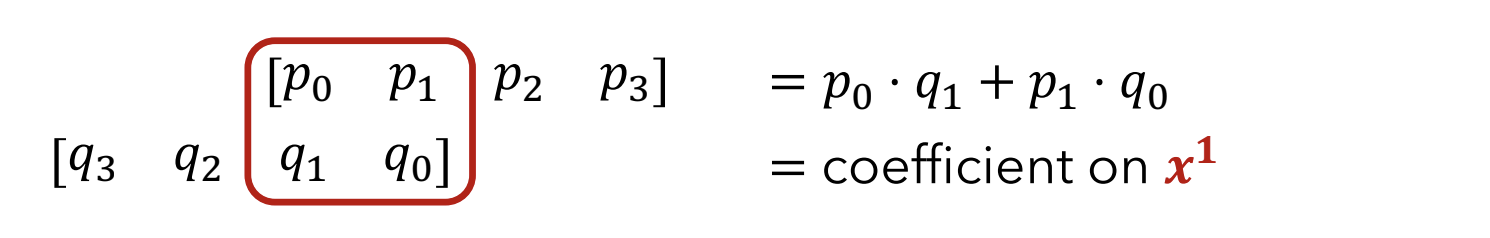
\includegraphics[scale=0.5]{cross-correlation.png}
		\end{center}
		This is called \textbf{cross-correlation}, and due to FFT, we can compute these in \( O(n \log n) \) time.   
	\item  \textbf{Integer Multiplication:} Say we wanted to multiply \( a = a_{n-1} \cdots a_2a_1a_0 \) and 
		\( b = b_{n-1}\cdots b_2b_1b_0 \). We can write down these two polynomials:
		\begin{align*}
			A &= a_0 + a_1x + a_2x^2 + \cdots + a_{n-1}x^{n-1}\\
			B&= b_0 + b_1x + b_2x^2 + \cdots + b_{n-1}x^{n-1} 
		\end{align*}
		and to compute the product, we can write \( A(x) \cdot B(x) \) and plug in \( x = 10 \). Naively we would think that 
		this takes \( O(n \log n) \) time, but this is not exactly true. This is because here, our additions and multiplications 
		don't exactly happen in \( O(1) \) time anymore, so we have to be careful! In fact, the multiplication can be as 
		large as \( \Theta(n) \). 

		After keeping track of all this, we get an \( O(n \log n \log \log n) \) algorithm. 
	\item \textbf{Fourier Transform:} FFT allows us to compute the Fourier transform of \( p(x) \) quickly -- we can decompose 
		 \( p(x) \) into its consistuent sines and cosines. There are too many applications of the Fourier transform to 
		 even list: 
		 \begin{enumerate}[label=\arabic*.]
		 	\item Music software
			\item Heart rate monitor
			\item Signal processing (e.g. cell phones)
			\item Many more!
		 \end{enumerate}
		 The fact that quantum computers can compute Fourier transforms exceedingly quickly is actually one of the main reasons 
		 that makes them so powerful.
\end{itemize}

	\section{Lecture 6}
\subsection{Clarification on BIBO Stability}
\begin{itemize}
	\item When we say a "bounded" signal, we mean that the amplitude of the signal is bounded at all times:
		\[
		|x(t)| < \infty \ \forall t \in \R
		\] 
		The same definition follows for discrete-time signals. 
	\item For LTI systems, we call the system BIBO stable if and only if its impulse \( h(t) \) is absolutely 
		integrable:
		\[
		\int_{-\infty}^{\infty} |h(t)| \diff t < \infty
		\] 
\end{itemize}
\subsection{Cross-Correlation}
\begin{itemize}
	\item The cross correlation between two signals \( r_{xy}(t) = r_{yx}(-t) \). To show this explicitly, we 
		look at the cross-correlation equation:
		\begin{align*}
			r_{xy}(t) &= \int_{-\infty}^{\infty} x(\tau)y(t + \tau) \diff \tau \\
			r_{yx}(t) &= \int_{-\infty}^{\infty} y(\tau) x(t + \tau) \diff \tau  
	\end{align*} 
	But for the second equation, we can define a \( \tau' = t + \tau\), so then we get: 
	\[
	r_{yx}(t) = \int_{-\infty}^{\infty} y(\tau' - t)x(\tau') \diff \tau' = \int_{-\infty}^{\infty} 
	x(\tau') y(-t + \tau') \diff \tau'
	\] 
	This looks like the first equation except we have \( -t \) instead of \( t \). Therefore, we have 
	\( r_{xy}(t) = r_{yx}(-t) \). The same works for discrete time: \( r_{xy}[n] = r_{yx}[-n] \). 
\end{itemize}

\subsection{More Convolution Properties} 
\begin{itemize}
	\item \textbf{Differentiation property:} Given \( y(t) = x(t) * h(t) \), then:
		\[
			\dv{t} y(t) = x(t) * \dv{h(t)}{t} = \dv{x(t)}{t} * h(t)
		\] 
	\item \textbf{Intergration Property:} Given \( y(t) = x(t) * h(t) \), we have:
		\[
		\int_{-\infty}^{t'} y(t) \diff  t = x(t) * \int_{-\infty}^{t'} h(\tau)\diff \tau 
		\] 
\end{itemize}
\subsection{Fourier Transform} 
\begin{itemize}
	\item The fourier transform came from the study of the heat equation, written as:
		\[
			c \rho \pdv{t} u(x, y, z, t) = k \left( \pdv[2]{x} + \pdv[2]{y} + \pdv[2]{z} \right) 
			u(x, y, z, t)
		\] 
		Fourier then claimed that the solution can be expanded in a series of sines with multiples of the variable. 
		In other word,s the solution is of the form:
		\[
		f(x) = \frac{1}{2a_0} + (a_1 \sin(x) + b_2 \cos(x)) + (a_2\sin(2x) + b_2\cos(2x)) + \cdots 
		\] 
	\item Recall the frequency response of an LTI system:
		\begin{center}
			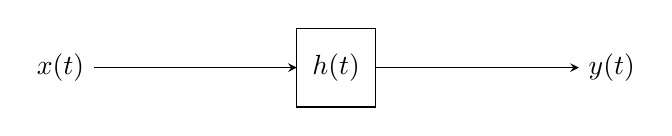
\begin{tikzpicture}
				\node (A) at (-3, 0) {\( x(t) \) };
				\node (B) at (4, 0) {\( y(t) \) };
				\draw[-stealth] (A) -- (0, 0);
				\draw (0, -0.5) rectangle node {\( h(t) \) } (1, 0.5);
				\draw[-stealth] (1, 0) -- (B);
			\end{tikzpicture}
		\end{center}
		Recall that we can characterize \( y(t) \) via a convolution: 
		\[
		y(t) = \int_{-\infty}^{\infty} x(\tau) h(t - \tau) \diff  \tau 
		\] 
		If we do this with our input \( e^{j 2 \pi ft} \), then we get:
		\[
		y(t) = H(f) e^{j 2 \pi ft} = H(\omega) e^{j \omega t }
		\] 
		Here, \( H(\omega) \) is defined to be the Fourier transfrm of the impusle response \( h(t) \):
		\[
			H(\omega) = \int_{-\infty}^{\infty} e^{- j \omega t} h(t) \diff t 
		\] 
		Alternatively, written in frequency language:
		\[
		H(f) = \int_{-\infty}^{\infty} e^{-j 2 \pi ft}h(t) \diff t 
		\] 
	\item Formally, the Fourier transform is defined as:
		\[
		H(f) \equiv \mathcal F \{h(t)\} \equiv \int_{-\infty}^{\infty} h(t) e^{-j 2\pi ft }\diff  t 
		\] 
		This transforms the signal \( h(t)  \) from the time domain into the frequency domain. The reason for this 
		is becuase the Fourier transform is a definite integral, which kills off any \( t \) dependence entirely. 
		In terms of angular frequency, we have:
		\[
		H(\omega) \equiv \mathcal F \{h(t)\} = \int_{-\infty}^{\infty} h(t) e^{-j \omega t}\diff t 
		\] 
	\item The inverse Fourier transform is:
		\[
			h(t) = \mathcal F^{-1} \{H(f)\} = \int_{-\infty}^{\infty} H(f) e^{j 2\pi ft}\diff  f 
		\]
		Since the Fourier transform takes objects from the time domain to the frequency domain, the inverse 
		Fourier transform takes things from the frequency domain to the time domain. 

		In terms of angular frequency, we have:
		\[
		h(t) = \mathcal F^{-1} \{H(\omega)\} = \frac{1}{2\pi}\int_{-\infty}^{\infty} H(\omega) 
		e^{j \omega t}\diff \omega 
		\] 
		This is also sometimes called the "synthesis equation", since we basically create \(  x(t) \) out of 
		\( H(\omega) \). 
	\item We can also provably show that the Inverse fourier transform does indeed invert the Fourier transform, 
		albeit with a lot of algebra. See lecture slides for the full derivation.  
	\end{itemize}

	\section{Lecture 7}
\subsection{DTFT and Convergence}
\begin{itemize}
	\item Not all functions have a Fourier transform, and the problem of whether a function has a Fourier 
		integral is an incredibly complex problem with no simple statement. 
	\item However, we know that there are several sufficient (but not necessary) conditions. Firstly, 
		we know that \( x(t) \) must be absolutely integrable. That is, 
		\[
		\int_{-\infty}^{\infty} |x(t)| \diff t < \infty
		\] 
\end{itemize}
\subsection{Fourier Transform Pairs}
\begin{itemize}
	\item There are several pairs of Fourier transforms that are useful to memorize.
	\item The Delta function:
		\[
			x(t) = \delta(t - t_0) \leftrightarrow X(f) = e^{-j 2\pi ft_0}
		\]
		This actually has strong implications about the nature of the Fourier transform -- there is an 
		"uncertainty principle" that manifests itself here. A signal cannot be both localized in time and frequency at
		the same time.
	\item Complex exponentials:
		\[
		x(t) = e^{j \omega_0 t} = e^{j 2 \pi f_0 t} \leftrightarrow X(f) = \delta(f - f_0)
		\] 
		This is the same as the previous point, except now we're going backwards.   
	\item Cosine functions:
		\[
		x(t) = \cos(2 \pi f_0 t) \leftrightarrow X(f) = \frac{1}{2}\delta(f - f_0) + \delta(f + f_0))
		\] 
		This makes sense: a plane wave is a composition of a left and right travelling wave.  
	\item Sine functions:
		\[
		x(t) = \sin(2 \pi f_0 t) \leftrightarrow X(f) = \frac{1}{2j}(\delta(f - f_0) - \delta(f + f_0))
		\] 
		Note that the only difference here is the minus sign, as a result of the conversion of sine into 
		complex exponentials.
	\item Shah function:
		\[
		x(t) = III(t) \leftrightarrow X(f) = III(f) \text{ or } X(\omega) = \frac{1}{2\pi}III(\omega)
		\] 
	\item Rect function:
		\[
		x(t) = \sqcap(t) \leftrightarrow \sinc(f)
		\] 
\end{itemize}

	\section{Fourier Transforms}
\subsection{Discrete Fourier Transform}
\begin{itemize}
	\item Recall the Shah function: \( x(t) = \text{III}(t) = \sum_{k = -\infty}^{\infty}\delta(t - k) \). Its 
		fourier transform in ordinary frequency is: 
		\[
		X(f) = \int_{-\infty}^{\infty} \sum_{k = -\infty}^{\infty} \delta(t - k) e^{-j 2 \pi f t}\diff t
		= \sum_{n = -\infty}^{\infty} \delta(f - n) = III(f)
		\] 
		So the Fourier transform of a Shah function is itself a shah function, in frequency space.  
	\item In Angular frequency (\( \omega \) ), then it's writtne as: 
		\[
		X(\omega) = X(f) = 2\pi \sum_{n = -\infty}^{\infty} \delta(2 \pi f - 2\pi n) = 2\pi \sum_{n = -\infty}^{\infty}
		\delta(\omega - 2 \pi n)
		\] 
\end{itemize}
\subsection{Convolutions and Fourier Transform} 
\begin{itemize}
	\item There is an identity between the Fourier transform and convolution, called the convolution theorem: 
		\[
		x_1(t) * x_2(t) \leftrightarrow X_1(f) X_2(f)
		\] 
		The right hand side can also be replaced by \( X_1(\omega) X_2(\omega) \), up to a normalization factor. 
		This equation basically says that the Fourier transform of the convolution of two function is also equal to the
		pointwise product of the Fourier transforms of \( x_1 \) and \( x_2 \). 

		\begin{proof}
			Start with the Fourier transform of \( x_1(t) * x_2(t) \) :
			\[
			\int_{-\infty}^{\infty} (x_1(t) * x_2(t)) e^{-j 2 \pi ft}\diff t = \int_{-\infty}^{\infty} \left( 
			\int_{-\infty}^{\infty} x_1(\tau) x_2(t - \tau) \diff \tau \right) e^{-j 2 \pi ft}\diff t 
			\] 
			Now, we take the \( t \) integral first becuase it's easier: 
			\[
			\int_{-\infty}^{\infty} x_1(\tau) \int_{-\infty}^{\infty} x_2(t - \tau) e^{-j 2 \pi ft}\diff t  \diff \tau
			= \int_{-\infty}^{\infty} x_1(\tau) e^{-j 2 \pi f\tau}X_2(f) \diff \tau = X_1(f) X_2(f) 
			\] 
		\end{proof}
	\item For example, consider the rect function \( \sqcap(t) \) that is 1 on the interval \( [-1 / 2, 1/2] \). 
		If we do the Fourier transform of this, we get a sinc function. At \( f = 0 \), we have 
		\( \sinc(f) = 1 \). 

		If we wanted to take the FT of the convolution of two rect functions, then we can use the convolution theorem 
		to conclude that \( \mathcal F(\sqcap(t)) = \sinc^2(f) \). Conversely, we know that the inverse Fourier 
		transform of \( \sinc^2(f) \) would be the triangular function, becuase we know that it's the convolution 
		of two rect functions.
\end{itemize}
\subsection{Fourier Series}
\begin{itemize}
	\item Consider a periodic function, where \( x(t) = x(t + nT) \). One way to write \( x(t) \) and also to 
		reflect its period, we can write it as a sum of delta functions: 
		\[
		x(t) = \sum_{n=-\infty}^{\infty} \left( x(t) \sqcap\left( \frac{t}{T} \right)  \right) * \delta(t - nT) 
		\] 
		Basically the rect function restricts the domain to only one period of \( x(t) \), and we convolve this with 
		a series of Delta functions in order to generate the roiginal fnction back. We can also do some simplifications
		on this: 
		\[
		x(t) = \left( x(t) \sqcap\left( \frac{t}{T} \right)  \right) * \sum_{n=-\infty}^{\infty} \delta(t - nT) 
		\] 
		Then we can use an identity to get: 
		\[
		x(t) = \left( x(t) \sqcap\left( \frac{t}{T} \right)  \right) \frac{1}{T}\text{III}\left( \frac{t}{T} \right) 
		\] 
		\question{How did we get the simplification of the delta sum into the Shah function?} 
	\item Turns out, if we perform a Fourier transform of \( x(t) \), then we get a discrete set of values, 
		also called a Fourier series. Taking the Fourier transform of the above function, and defining 
		\( g(t) = x(t) \sqcap(t / T) \), then we can write: 
		\begin{align*}
			\mathcal F \{x(t)\} &= \mathcal F \left\{g(t) * \frac{1}{T}\text{III}\left( \frac{t}{T} \right) \right\}  \\
								&= \mathbf G(f) \text{\textbf{III}} (Tf)
		\end{align*}
		where \( \mathbf G(f) \) is the Fourier transform of \( g(t) \).  Expanding the Shah function out, we 
		have: 
		\[
		\frac{1}{T}\sum_{n=-\infty}^{\infty} \mathbf G(f) \delta\left( f - \frac{n}{T} \right) 
		\] 
		The delta function will select \( f = \frac{n}{T} = nf_0\), so we get: 
		\[
		\frac{1}{T}\sum_{n=-\infty}^{\infty} G(nf_0) \delta\left(f - \frac{n}{T}\right)
		\] 
	\item So, from here we can conclude that the Fourier transform of a periodic function is just a series over that 
		function. 
	\item The inverse Fourier transform used to be:
		\[
		x(t) = \int_{-\infty}^{\infty} \mathbf X(f) e^{j 2 \pi ft}\diff f 
		\] 
		Where \( \mathbf X(f) \) is the (continuous-time) Fourier transform of \( x(t) \). Since \( x \) is periodic, 
		then we can write
		\begin{align*}
			x(T) &= \int_{-\infty}^{\infty} \sum_{n=-\infty}^{\infty} \mathbf G(n) \delta\left( f - \frac{n}{T} \right) 
		e^{j 2 \pi ft }\diff  f\\
		&= \frac{1}{T}\sum_{n=-\infty}^{\infty} \mathbf G(n) \int_{-\infty}^{\infty} \delta\left( f - \frac{n}{T} \right) e^{j 2 \pi ft} \diff  f  \\
		&= \frac{1}{T}\sum_{n=-\infty}^{\infty} \mathbf G(n) e^{2 \pi \frac{n}{T}t}\\
		&= \frac{1}{T}\sum_{n=-\infty}^{\infty} \mathbf G(n) e^{j 2 \pi n f_0 t} 
		\end{align*} 
		Note that the delta function only picks out the frequency \( \frac{n}{T} \), which allows us to get a discrete
		sum of frequencies. This is called the Discrete Fourier Series. 
\end{itemize}

	\section{CNNs, ResNets, Batch Normalization}
\subsection{Summary of Last Lecture}
\begin{itemize}
	\item The structure of a neural network: we described the mathematical structure
		of a neural network and how each neuron behaves at every step:
		\begin{align*}
			a_j^{(\ell)} &= \sum_{i \in [d_{\ell - 1}]} \theta_{ji}^{(\ell)}x_i^{(\ell
			- 1)}\\
			x_j^{(\ell)} &= g_\ell(a_j^{(\ell)}) 
		\end{align*}
	\item For maximum likelihood learning, we denote the total loss as the sum of the
		individual losses: 
		\[
			\mathcal{L}(\theta) = \sum_i \mathcal{L}_i(\theta) = \sum_i
			\mathcal{L}(f_{\theta}(x_i), y_i)
		\]
	\item Stochastic Gradient Descent (SGD): in its purest form, defined by the
		updates
		\[
			\theta_{t + 1} = \theta_t - \epsilon_t
			\nabla_{\theta_t}\mathcal{L}(\theta_t)
		\]
		where we select an \( \epsilon_t \) at random at each iteration \( t \). 
	\item Backpropagation: we learned of an \( O(m) \) algorithm to calculate the
		gradient of the loss throughout the neural net:
		\[
			\Delta_j^{(\ell)} = \left( \sum_{k \in [d_{\ell + 1}]} \Delta_k^{(\ell +
			1)} \theta_{kj}^{(\ell + 1)} \right)g'(a_j^{(\ell)})
		\]
\end{itemize}
\subsection{Convolutional Neural Networks (CNN)}
\begin{itemize}
	\item Firstly, fully connected neural networks are parameter hungry. Usually,
		too many parameters leads to overfitting of the data, which we know to be
		suboptimal.
	\item The motivation for CNNs comes from our desire to incorporate our "inductive
		bias" into the neural net. Inductive bias is our desire to force the neural
		network to learn certain aspects about the data. 

		In our naive approach, if we wanted to forcefully change some parameters \(
		\theta \), then the network would respond in an unpredictable way because of
		its complexity. So, in order to control the neural networks in a way, we turn
		to convolutional neural networks.  
\end{itemize}

\subsubsection{Invariance and Equivariance}
\begin{itemize}
	\item They are both defined with respect to a particular transformation.
	\item As an example, consider a translation \( T \):
		\[
			\begin{tikzcd}[sep = 30]
				x \arrow[r] \arrow[d, "f_\theta"] & T(x) \arrow[d, "f_\theta"] \\
				f_{\theta}(x)  &  f_\theta(T(x))	
			\end{tikzcd}
		\]
		the idea is that with our classification, we would like to have \(
		f_\theta(x) = f_\theta(T(x)) \). In this case, we call this
		\textbf{invariance.}
	\item On the other hand, if we have \( f_{\theta}(T(x)) = T(f_{\theta}(x)) \),
		then this operation is called \textbf{equivariance}. 

		In general, because the spaces (dimensions) in which \( x \) and \( T(x) \)
		live in may be different, what we really want in general is:
		\[
			f_{\theta}(T_x(x)) = T_y(f_{\theta}(x))
		\]
		In the case where \( T_x = T_y \) we have the earlier form. 
\end{itemize}
\subsubsection{Structure of a CNN}
\begin{itemize}
	\item In a CNN, the operation from each layer to the next is a convolution, and
		no longer a dot product between the vector \( \theta \) at layer \( \ell \)
		and your weights. That is, 
		\[
			a^{(1)}(i_1, i_2) = \sum_{j_1 \in [F]} \sum_{j_2 \in [F]} x^{(0)}(i_1 +
			j_1, i_2 + j_2) \theta(j_1, j_2)
		\]
		so now, \( \theta \) is a 2-dimensional kernel we use to compute the
		convolution. This also means that each neuron is only connected to the
		neurons in the previous layer by the size of the convolution only.    

		\question{what does the bias actually mean in this case then? Is it some
		constant matrix \( \theta_0 \)?}

		\answer{No, you do the convolution as normal, then add a bias \( b \) at the
		very end.}
	\item Note that the filter at each layer doesn't have to be the same. If you were
		processing an image, one filter could be a horizontal gradient, and the other
		could be a vertical gradient. This is allowed.  
	\item In the case of image processing, you may also need to take your
		convolutions channel-wise because your input is RGB.  
	\item In general, visualizing the first layer of your network is relatively easy,
		because it's just a collection of the images you've learned.

		\question{Is the first layer the output layer or the first layer through your
		convolution?}
	\item Some technical terms related to neural nets: 
	\begin{itemize}
		\item \textbf{Padding:} When you do convolution on the edges, you may need to pad
			the edges with zeros (or some other value) so that the kernel completely
			overlaps with your matrix. In general, convolving a \( (W \times W) \) matrix
			with an \( (F \times F) \) filter, then you get a \( (W - F + 1)
			\)-dimensional matrix. 
		\item \textbf{Pooling:} You take the elements in a certain window of the matrix
			(say, the top left), and take the value according to some defined function.
			In the case of max-pooling, you take the max value, for example. 
	\end{itemize}
	\item When we finish training our model using SGD (or other methods), we can then
		look at the learned model by computing \( \nabla_x a_i^{(\ell)}(x;
		\hat{\theta}) \). Basically, we are looking for the behavior of the neural
		net to small changes in the data. 
	\item One thing we find when training neural networks is that the depth of the
		neural net doesn't always lead to a better result, and is a result of the
		vanishing gradient. 

		\question{What is this vanishing gradient really mean here?} 

		\answer{Consider logistic regression, where your activation function is the
			sigmoid. You want to maximize the probability, which forces you to be in
		a regime where there are very small gradients. So, you hit a wall.}


		\comment{Aside on vanishing gradients:
			Consider a function:
			\[
				f(x) = \left( \prod_{i = 1}^{n}w_i \right)x
			\]
			and you have individual gradients:
			\[
				\pdv{\mathcal{L}}{w^{(2)}} 
				= \pdv{\mathcal{L}}{x^{(3)}}
				\pdv{x^{(3)}}{w^{(2)}}
		\]
	The reason vanishing gradients happen is because you multiply many of these terms
together -- and as a result, you're getting a \textit{really} small term, and this
leads to vanishing gradients.}
\end{itemize}

\subsection{ResNets}
\begin{itemize}
	\item One way to deal with the limitations of neural networks is to use "skip
		connections", or basically connect the previous layer directly to the next
		layer. That is, we have:
		\[
			x^{(\ell + 1)} = \mathcal{F}_{\ell + 1}(x^{(\ell)}) + x^{(\ell)}
		\]
		compared to what we had before (only the \( \mathcal{F}_{\ell +
		1}(x^{(\ell)}) \) the residual \( x^{(\ell)} \) term (not sure)

		\question{so what does the residual term do that allows you to bypass the
		learning barrier?} 

		\answer{It solves the issue of vanishing gradients, because the gradient of
		the last step directly influences the first step.} 
	\item As a result, deeper ResNets actually do perform progressively better.    
\end{itemize}

\subsection{Batch Normalization}
\begin{itemize}
	\item When you want to train a neural net, and you don't want inputs from
		different layers of the network to be in different ranges. Because of the way
		backpropagation works (each next layer is dependent on the previous one),
		then you'd like all the gradients and networks to live in similar ranges so
		that you don't get random spikes for no reason.
	\item To accomplish this, you normalize each hidden layer in the same way you
		normalize the input data! That is, in each batch, we can compute the
		statistics of the batch:
		\[
			\mu_B = \frac{1}{n}\sum_{i \in [b]} x_i, \quad \sigma_B = \frac{1}{n}
			\sum_{i \in [b]}(x_i - \mu)^2
		\]
		then normalize each layer based on the statistics of the batch. That is, for
		each node in the neural network, we then have:
		\[
			x^{(\ell)} \leftarrow \frac{x^{(\ell)} - \mu_B}{\sigma_B + \epsilon}
		\]
		this normalizes each \( x^{(\ell)} \) in each batch so make sure that the
		ranges are consistent across each layer. \question{Remember: this is done at
			\textit{every layer}, so you compute \( \mu_B \) and \( \sigma_B \) for
		each layer, and normalize it.} 
	\item You also want to augment \( x^{(\ell)} \) by learned \( \gamma, \beta \):
		\[
			x^{(\ell)} \leftarrow \gamma x^{(\ell)}+ \beta
		\]
		\question{and why do you do this?}

		\answer{Don't worry about it, it's not important.}
\end{itemize}

	\section{Zero Sum Games}
\subsection{Game 1}
\begin{itemize}
	\item We saw last time that given a ZSG structured like this:
		\begin{center}
			\begin{tabular}{c|c|c}
				& P1& P2\\
				\hline 
				P1 & 3 & -1\\
				\hline
				P2 & -2 & 1
			\end{tabular}
		\end{center}
		then we can calculate that the payoff for column 1 is \(3p_1 - 2p_2\), and the payoff for column 
		2 is \(-p_1 + p_2\).
	\item This meant that the column player's best strategy was to look at these two values, and minimize this.  
	\item The row player will then pick \(p_1, p_2\) in order to maximize what the column player tries to 
		minimize. Therefore, the row player wants to calculate:
		\[
			\max_{\text{mixed strategies \(p\)}} \{\min \{3p_1 - 2p_2, -p_1 + p_2\} \} 
		\] 
	\item As we said last lecture, this can be solved using LP! We'll also see that the row player going 
		first doesn't hurt them. 
	\item So we can formulate our LP as follows:

		Maximize a quantity \(z\), subject to the constraints:
		\begin{align*}
			z & \le 3p_1 - 2p_2\\
			z &\le -p_1 + p_2\\
			1 &= p_1 + p_2\\
			0 &\le p_1, p_2
		\end{align*}
		Note that \(z = \min \{3p_1 - 2p_2, -p_1 + p_2\} \), so by maximizing \(z\) subject to these two 
		constraints means that \(z\) is constrained to the smaller of these two. 
\end{itemize}
\subsection{Game 2}
\begin{itemize}
	\item The exact same game board, except we allow the column player to go first and the row player goes 
		second. 
		\begin{center}
			\begin{tabular}{c|c|c}
				& P1& P2\\
				\hline 
				P1 & 3 & -1\\
				\hline
				P2 & -2 & 1
			\end{tabular}
		\end{center}
	\item We do the exact same thing, by considering the possibilities from the row player's perspective. This
		is the same as looking from the column player's perspective in the previous problem. 
		\begin{itemize} 
			\item From the row player's perspective, payoff of row 1 is \(3q_1 - q_2\), and row 2 is: 
				\(q_2 - 2q_1\). So we want to choose the max of these two, i.e.:
				\[
				\max \{3q_1 - q_2, -2q_1 + q_2\} 
				\] 
			\item The column player will try to minimize this score, so they'll want to choose:
				\[
					\min_{\text{mixed strategies \( q\)}} \{ \max \{3q_1 - q_2, -2q_1 + q_2\} \} 
				\] 
		\end{itemize}
	\item This is another linear program! Here, we want to minimize \(z\), subject to:
		\begin{align*}
			3a_1 - a_2 &\le  z\\
			-2q_1 + q_2 &\le z\\
			q_1 + q_2 &=  1 \\
			q_1, q_2 &\ge 0
		\end{align*}
		Again, note that \(z\) is equal to the larger of the two inequalities, using the same logic as 
		before.
	\item Now we compare the two problems, and compare the final quantities that we wanted to compute. 
		\begin{itemize}
			\item In game 1, we wanted to find \(\max_p \{\min_q \{S(p, q)\} \} \) 
			\item In game 2, we wanted to find \(\min_q \{\max_p \{S(p, q)\} \} \)
		\end{itemize}
	\item Given this construction, we have the inequality
		\[
		\max_p \{\min_q \{S(p, q)\} \} \le \min_q \{\max_p \{S(p, q)\} \} 
		\] 
		
		\question{If the dual of the dual is the original, doesn't this mean that we get a situation like 
		\(x \le  y \le  x\)?}

		\answer{No, becuase the inequality flips again, so we get \( x \le y \ge  x \), a valid inequality.}     

		The best way to see that this is true is that it's always better to be the player that 
		goes second. Therefore, finding the minimum over \(q\) is better because they're able to ``react'' to 
		the column player's moves.
	\item It turns out that these two LPs are actually duals of each other (the proof is to construct 
		the second LP from the first one). Now, recall the property of strong duality, which holds for any LP
		that is bounded. This game is clearly bounded, so we know that there is an optimal value of the game 
		(denoted by $\mathrm{Value}(\text{game})$) is the same for both games!  

		This is called the \textbf{min-max theorem.}
	\item This tells us that the order of play doesn't change the value of the game, and there is an optimal 
		probability distribution that the row player can choose without caring about what the column player 
		does. 
		
		\comment{Note that this is a zero sum game not by the game table, but because the gain of one player 
		is an equal loss in the other player. So the numbers in the table can be anything!} 
	\item This also says that all zero sum games are strongly dual.
\end{itemize}
\subsection{P vs. NP}
\begin{itemize}
	\item So far, we've seen a lot of algorithms: polynomial multiplication, MSTs, APSP, etc.
	\item In theoretical CS, we consider all these problems to be ``efficiently solvable,'' We define 
		this to be the case when a problem can be solved in \textbf{polynomial time.}

		\comment{This is only in theoretical CS. In practice, we'd want to get everything down to 
		\(O(n)\) time, if possible. Even \(O(n^2)\) is quite bad, since given an input of size 
		\(10^9\) (as is the case with the facebook graph), then the computation is on the 
		order of \(10^{18}\) (very bad)!}
	\item We define P (stands for polynomial) to be a set of computational problems that are considered to be
		efficiently solvable.  
	\item We define NP (stands for non-polynomial) to be another complexity class that aren't 
		efficiently solvable themselves, but whose 
		solutions can be efficiently checked. 
		\begin{itemize}
			\item Example: 3-coloring problem. We want to find a 3-coloring on this graph. Naively, 
				we can brute-force and try all possible combinations, which would correspond to checking 
				\(3^{n}\) possible graphs. 
			\item The best known algorithm for this solves the problem in \(1.3289^{n}\) time.  
			\item So this algorithm is not in P, but it is in NP, since any solution can be verified in 
				polynomial time (by checking all edges)
			\item Example 2: Factorization. Given an \(n\)-bit integer \(N\), we want to factorize it into 
				two numbers \(p, q >1\) such that $pq = N$. 
			\item Naively, we can divide \(N\) by every number from \(1\) to \(\sqrt{N} \). In terms of 
				time complexity, this is \(O(\sqrt{N} )\), which we can simplify this to \(O(2^{n /2}\) due to 
				the way numbers are represented as bitstrings. 

				The best algorithm runs in time \(C^{n^{1/3}} \log(n)^{2/3}\), so this is not a problem 
				that's known to be in P. 

				However, the problme is in NP, because we can just verify any solution by multiplying them 
				together, which takes at most \(O(n^2)\) time. 
		\end{itemize}
\end{itemize}

	\section{Transfer Function of LTI Systems}
\begin{itemize}
	\item For an LTI system with the standard input and output pairs, we know that since \( y(t) = x(t) * h(t) \), 
		then this means that 
		\[
		Y(s) = X(s) H(s)
		\] 
		where \( H(s) \) denotes the Laplace transform of the impulse response, 
		\[
		H(s) = \int_{-\infty}^{\infty} h(t) e^{-st}\diff t 
		\] 
	\item For an LCCDE of the form:
		\[
			\sum_{k=0}^{N} a_k \dv[k]{y(t)}{t} = \sum_{k=0}^{M} b_k \dv[k]{x(t)}{t}
		\] 
		then we can take the Laplace transform of both sides, 
		\[
		\sum_{k=0}^{N} a_k s^{k}Y(s) = \sum_{k=0}^{M} b_k s^{k}X(s)
		\] 
		So, this means that:
		\[
		H(s) = \frac{Y(S)}{X(s)} = \frac{\sum_{k=0}^{\infty} b_k s^{k}}{\sum_{k=0}^{N} a_k s^{k}}
		\] 
\end{itemize}
\subsection{RLC Circuit}
\begin{itemize}
	\item Consider the following circuit:
		\begin{center}
			\begin{circuitikz}[american]
				\draw (0, 3) to [voltage source, l_ = \( x(t) \)] (0, 0);
				\draw (0, 3) to [R] (2, 3) to [R] (4, 3);
			\end{circuitikz}
		\end{center}
\end{itemize}
\subsection{Effect of Poles}
\begin{itemize}
	\item For non-repeated poles (as in, the poles aren't degenerate), then the transfer function can 
		be written generically as:
		\[
		H(s) = \sum_{i=1}^{N} \frac{A_i}{s - a_i}
		\] 
		If the system is causal, then recall that for an LTI system this means that \( h(t) = 0 \) for \( t < 0 \)
		\[
		h(t) = \sum_{i=1}^{N} A_i e^{-a_i t}u(t)
		\] 
	\item If \( \alpha_i \) is repeated \( m \) times, then the system response will include these terms:
		\[
			t^{m-1}e^{\alpha_i t}, \cdots,te^{\alpha_1}t, e^{\alpha_i t}
		\] 
\end{itemize}
\subsection{Stability of Causal System}
\begin{itemize}
	\item Given a causal system described by  \( H(s) \), we saw earlier that \( Y(s) = H(s) X(s) \). There's also 
		a theorem that says that the system is stable if and only if all poles of \( H(s) \)  have strictly negative 
		real parts. 
		This is because of two reasons:
		
		\begin{enumerate}[label=\arabic*.]
			\item This is because if \( H(s) \) is rational, 
				then the causality is equivalent to the region of convergence to 
				the right of the rightmost pole (on the real line)
			\item The absolute integrability condition \( \int_{-\infty}^{\infty} |h(t)|\diff t < \infty \) means 
				that the imaginary axis is within the ROC. 
		\end{enumerate}
\end{itemize}
\subsection{Connected LTI Sytems}
\begin{itemize}
	\item For systems connected in series, then \( H(s) = H_1(s)H_2(s) \), and in parallel then
		\( H(s) = H_1(s) + H_2(s) \). This is the exact same as the Fourier transform \( H(\omega) \) properties. 
	\item For feedback control systems (e.g. a compensator), then we define an error function 
		\( E(s) = X(s) - H_2(s) Y(s) \). The subtraction comes from the fact that the feedback is fed 
		as a minus sign. Then, \( Y(s) = H_1(s) E(s) \), and solving both equations 
		gives:
		\[
		Y(s) = H_1(s) X(s) - H_1(s) H_2(s) Y(s) \implies H(s) = \frac{Y(s)}{X(s)} = \frac{H_1(s)}{1 + H_1(s)H_2(s)}
		\] 
\end{itemize}
\subsection{Z-transform}
\begin{itemize}
	\item Very much the same as the Laplace transform, but for discrete-time signals. 
	\item This is very similar to the DTFT formula:
		\[
			X(e^{j \omega}) = \sum_{n=-\infty}^{\infty} x[n] e^{-j \omega n}
		\] 
		This is periodic because the signal is discrete in time. The z-transform is the generalized version of this 
		formula, written as:
		\[
			X(z) = \sum_{n=-\infty}^{\infty} x[n] z^{-n}, z \in \C
		\] 
		so really, the only difference is that we swapped \( e^{-j \omega} \) for a general complex 
		number \( z \). Because \( z \) also has a magnitude term, there's also a corresponding region of 
		convergence for \( z \). 
\end{itemize}
\subsection{Pairs}
\begin{itemize}
	\item Given \( x[n] = \delta[n] \), then:
		\[
			X(z) = \sum_{n=-\infty}^{\infty} \delta[n] z^{-n} = 1
		\] 
		as long as \( z \neq 0 \). With that caveat in mind, the ROC is the entire complex plane. 
	\item Given \( x[n] = a^{n}u[n] \):
		\[
			X(z) = \sum_{n=-\infty}^{\infty} a^{n}u[n] z^{-n} = \sum_{n=0}^{\infty} a^{n}z^{-n}
			= \sum_{n=0}^{\infty} (az^{-1})^{n} = \frac{1}{1 - (az^{-1})}
		\] 
		the last step simplifies due to geometric series. The condition for this to converge is 
		that \( |az^{-1}| < 1 \), since that's when the geometric series converges. So this simplifies 
		to \( |z| > |a| \), or \( |z| > a \) since \( a \) is real. 

		Visually, this corresponds to a boundary at infinity and one that's a circle at radius \( a \). Consequently, 
		if the unit circle exists within the region of convergence, then we know that the DTFT of the signal 
		exists. 
	\item Given \( x[n] = -a^{n}u[-n - 1] \):
		\[
			X(z) = \sum_{n=-\infty}^{\infty} -a^{n}u[-n - 1] z^{-n} = \sum_{n=-\infty}^{-1} -a^{n}z^{-n}
			= 1 - \sum_{n=0}^{\infty} (-a^{-1}z)^{n}  = 1 - \frac{1}{1 - a^{-1}z}
		\] 
		The region of convergence is defined similarly: \( |za^{-1}| < 1 \), so \( |z| < |a| \). This is just a
		filled circle up to a radius of \( |a| \). Of course, the DTFT exists only when the radius of this circle 
		is larger than 1. 
	\item Given  \( x[n] = -\left( \frac{1}{2} \right)^{n}u[-n - 1] + \left( -\frac{1}{3} \right)^{n}u[n] \), 
		since the z-transform is linear, then:
		\[
		X(z) = \frac{1}{1 - 2z } + \frac{1}{1 + z^{-1} / 3} = \cdots = \frac{6z^2 - 6z - 1}{(3z + 1)(2z - 1)}
		\] 
\end{itemize}
\subsection{Z-transform properties}
\begin{itemize}
	\item The ROC for z-transforms are circles or rings instead of planes, and that's just becuase we're 
		converting \( e^{j \omega} \) to \( z \). 
	\item See the lecture slides for a table on the properties. 
\end{itemize}
\subsection{Inverse Z-transform}
\begin{itemize}
	\item We can compute the inverse Z-transform using partial fraction expansion. The reason we keep going back 
		to this is because many Z-transforms are characterized by rational functions, so if we can find a way to 
		split the fractions up then we can find the inverse from linearity.  
\end{itemize}





	\section{Quantum Computing Platforms}
\begin{itemize}
	\item Trapped ions: qubits are single atoms, but we've removed one of the electrons so they're positively charged.
		We do this so that we have better control over them. This is the platform that's pursued by Honeywell/
		Quantinuum, AQT, among other companies.  

		\textbf{Pros:}
		\begin{itemize}
			\item These have long coherence times \( T_2 \sim 1 \) minute
			\item They operate at room temperature -- basically it's just a big vaccuum chamber sitting in a room 
				without the need for cryogenics. Nothing about the qubits require low temperature, we just happen 
				to involve cryogenics in order to achieve a better vaccuum. 
			\item Highest fidelity gates so far, and have been one of the first to discover quantum gates.  
		\end{itemize}

		\textbf{Cons:}
		\begin{itemize}
			\item Gates operate typically at 50 microseconds.  
			\item Requires lasers, optics
			\item The coulomb interaction between ions makes scaling more difficult
		\end{itemize}
	\item Neutral Ions: basically the same trapping techniques, except the atoms are neutral instead of 
		charged. We can't trap them using fields because they are neutrally charged. 

		\textbf{Pros:}
		\begin{itemize}
			\item Long qubit coherence times
			\item Room temperature operation 
			\item Inherently somewhat scalable, since neutral atoms don't interact
			\item Optical interface. 
		\end{itemize}
		\textbf{Cons:}
		\begin{itemize}
			\item Experiments usually looks like a mess (requires a lots of lasers), and much of the effort goes into 
				managing the lasers
			\item Requires an ultrahigh vaccuum (so we need cryogenics basically)
			\item Trapping is inherently more difficult and requires high laser power 
		\end{itemize}
	\item Superconducting qubits: these are man-made qubits instead of atoms. 

		\textbf{Pros}
		\begin{itemize}
			\item Chip-based architecture. It's something that we can imagine scaling up to a chip, and we interact 
				with it electronically
			\item Fast gate times (on the order of 50 nanoseconds)
			\item Previously leading the field commercially, but starting to recognize that superconducting 
				qubits might not be the way. (some comapnies are starting to invest in atomic-based approaches)  
		\end{itemize}

		\textbf{Cons:}
		\begin{itemize}
			\item Requires dilution refrigerators, so need cryogenic temperatures 
			\item Short coherence times, though this is getting much better 
			\item Control lines needed for every individual qubit -- every single qubit you want to add means an 
				extra set of lines you need to connect to your system. 
			\item Not very anharmonic. 
		\end{itemize}
	\item Quantum Dots: creating a 2D electron gas, and is possibly the most similar to the structure that we studied 
		in the previous lecture. 
		
		\textbf{Pros:}
		\begin{itemize}
			\item Semiconductor chip based architecture
			\item High fidelity, fast-qubit and two qubit gates. 
			\item Controlled by microwaves and electronics, there are no lasers required in this process. 
		\end{itemize}
		
		\textbf{Cons:}
		\begin{itemize}
			\item Requires cryogenic temperatures
			\item Short coherence times 
			\item Lots of tuning required for each device -- very sensitive architecture
			\item Scaling up to many qubits is still an open problem. We can do 2-qubit gates, but it's not clear 
				how we would scale up beyond that. 
		\end{itemize}
	\item Photonics: none of the stuff that we've talked about so far really applies here. States are single 
		photons, where the information is either stored in the polarization or which rail the photon 
		lives on. 
		
		\textbf{Pros:}
		\begin{itemize}
			\item Silicon chip based architecture
			\item Room temperature operation, what this basically means is that in principle we can do this 
				at room temperature, but the best photon detectors still require cryogenics. 
			\item Fairly easy to scale up, since photons naturally fly around
			\item "Measurement" based -- some of the gates are very easy to physically implement. For instance, 
				if you wanted to change the polarization then all you'd do is just introduce a wave plate
		\end{itemize}
		
		\textbf{Cons:}
		\begin{itemize}
			\item Gate operations are very difficult to achieve, and are inherently probabilistic. Preparing 
				the state itself is a challenge (trying again and figuring out when you succeed), then performing 
				the desired computation afterwards. 
			\item Requires identical photonic states and photonic elements
			\item Low gate fidelities
		\end{itemize}
\end{itemize}
\subsection{Trapped Ions}
\begin{itemize}
	\item Ideally we'd like to use the simplest atom possible, which in our case would be hydrogen-like 
		atoms. We can't use hydrogen itself, because transitions for hydrogen are in the UV spectrum, which poses 
		some challenges (what specifically?)
	\item Commercially, we normally use alkaline earth metals and then strip one electron off so that we end up with 
		a hydrogen-like atom. 
	\item Hydrogen-like atoms have a principal quantum number \( n \), whose energy scales with:
		\[
		E_n = -\frac{z^2 \frac{\mu}{m} E_H}{2n^2}
		\] 
		\( E_H \) is a physical constant, which is written as \( E_H = mc^2 \alpha^2 \)
	\item We also have angular momentum \( \ell \), which has possibilties between \( 0 \) to \( n - 1 \). 
	\item Transitions between these obey selection rules, which tells us that \( \Delta \ell = \pm 1 \) and 
		\( \Delta m = \pm 1 \). 
\end{itemize}

\end{document}
